\documentclass[11pt]{llncs}

\usepackage{graphicx}
\usepackage{parskip}
\usepackage{url}

\usepackage{listings}
\usepackage{color}

\definecolor{dkgreen}{rgb}{0,0.6,0}
\definecolor{gray}{rgb}{0.5,0.5,0.5}
\definecolor{mauve}{rgb}{0.58,0,0.82}

\lstset{frame=tb,
  aboveskip=1em,
  basicstyle={\small\ttfamily},
  belowcaptionskip=0.5em,
  belowskip=1em,
  breaklines=true,
  breakatwhitespace=true,
  captionpos=b,
  columns=flexible,
  commentstyle=\color{dkgreen},
  frame=single,
  keywordstyle=\color{blue},
  language=C,
  numbers=left,
  numberstyle=\tiny\color{gray},
  showstringspaces=false,
  stringstyle=\color{mauve},
  tabsize=3
}

\usepackage{loblib}

\newcommand{\flushreload}{\textsc{Flush}+\textsc{Reload}}
\newcommand{\litem}{\item[\lobclaw{simple}] }

\begin{document}

\title{PLUNGER: Reproducing FLUSH+RELOAD: A High-Resolution, Low-Latency Side
Channel Attack On GnuPG}
\author{Daniel Ge \and David Mally \and Nicholas Meyer}
\institute{University of Pennsylvania}
\maketitle

\lobwatermark

\begin{abstract}

    In their paper, Yarom and Falkner\cite{YF13} presented a side channel
    attack, named \flushreload{}, on the L3 caches of Intel x86 processors. The
    attack takes advantage of content-based memory page sharing between
    non-trusting processes to monitor memory accesses of a victim process. This
    technique can be used on GnuPG pre-1.4.14 to identify the binary sequence of
    an RSA private exponent by discerning which branches are taken.

    In this paper, we demonstrate an implementation of the \flushreload{}
    technique and apply it on a few platforms. Confirming the results from the
    original paper, the attack works on Linux platforms. While OS X was never
    mentioned in the original paper, the attack appears to be feasible on the
    platform.

\end{abstract}

\section{Background}
\subsection{Caches}

In modern computer architectures, processors often have a system of caches to
store recently-used data for efficient access. Caches are essentially small,
fixed-size blocks of SRAM that act as a hash table. However, rather than using a
hashing scheme such as separate chaining or linear probing, caches
\textit{replace} data upon collision, necessitating a slow lookup to system
memory when a collision, or \textit{cache miss} occurs. When data misses in the
cache, the processor must stall and wait for the data to arrive, a very slow
operation. While a cache lookup may take as little as 0.5 nanoseconds, a cache
miss that goes all the way out to system RAM may take as long as 50ns, 100 times
slower.

A typical cache architecture is laid out in three levels, generally referred to
as the \textit{L1}, \textit{L2}, and \textit{L3}. The L3 cache is usually larger
than than the L2, which itself is usually larger than the L1; L1 and L2 caches
are also generally allocated on a per-core basis in the case of multi-core CPUs,
whereas the L3 cache is usually shared between all cores.  L1 caches are also
typically divided into \textit{instruction} sections and \textit{data} sections,
each reserved for that particular type of instruction.  It is equally important
for instruction memory as well as data memory to be cached, as both require fast
access in order for the CPU to be performant. For example, the Intel Haswell i7
4600U CPU has a 128KiB L1 cache, divided into two 64KiB caches for instructions
and data; a 512KiB L2 cache, and a 4MiB L3 cache.

Naturally, a cache closer to a core has a lower access latency because the core
has to traverse fewer buses. On Intel architectures, the caches are considered
\textit{inclusive}, meaning that whatever data is contained in a core's L1 cache
will also be contained in the core's L2 cache and the CPU's L3 cache.
Therefore, when data are evicted from the L3 cache, they will also be evicted
from the L2 and L1 caches.

\begin{figure}[h]
    \setlength\fboxsep{0pt}
    \setlength\fboxrule{0.5pt}
    \centering
    \fbox{
        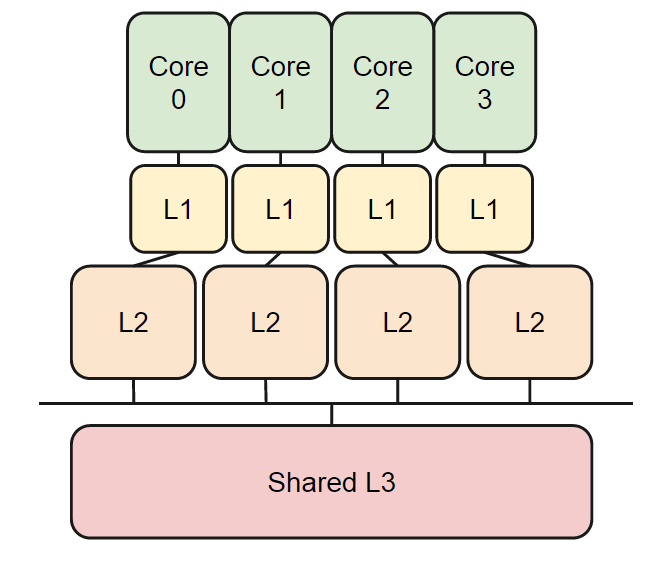
\includegraphics[scale=0.4]{img/caches}
    }
    \caption{Typical CPU Cache Architecture}
\end{figure}

\subsection{Page sharing} % David

Modern operating systems also implement a technique known as \textit{page
sharing}, which helps reduce the memory footprint of running processes by
avoiding redundant replication of memory pages. Page sharing may also be used as
an efficient, safe channel between two co-operating processes.

Windows, Linux, and possibly OS X\footnote{It is unclear whether or not OS X
implements page deduplication, but as far as we can tell it does} also perform a
more aggressive form of page sharing known as \textit{page deduplication}. With
this scheme, the operating system scans memory pages during idle CPU cycles, and
looks for pages that are identical in content. It collapses those pages into a
single page that is then shared by all processes that were accessing those
identical pages. As a result of this page deduplication scheme,
processes may be unknowingly or unintentionally sharing memory with one another.
However, to prevent malicious access to the shared pages, the operating system
maps shared pages as copy-on-write; that is, when a process wishes to write to a
page, it must first make a local copy for itself that it can safely modify. When
a write is requested, the CPU traps to the kernel, which then remaps a copy of
the desired page for the process requesting the write, and then returns control
to the calling process. Read operations in this scheme are safe, as they do not
modify the targeted page.

\subsection{RSA}

RSA is a standard cryptosystem for public key encryption. The scheme works as
follows. Choose two distinct prime numbers, $p$ and $q$.

\begin{enumerate}
    \item Compute $N = pq$.
    \item Compute $\phi(N) = \phi(p)\phi(q) = (p-1)(q-1)$
    \item Choose $e, 1 \leq e \leq \phi(N)$, where $gcd(e,\phi(N)) = 1$.
    \item Compute $d = e^{-1}\ mod\ \phi(N)$
    \item Let the private key be $(d,N)$ and the public key be $(e,N)$
\end{enumerate} 

Encryption can be performed by calculating $c = m^e\ mod\ N$. Likewise,
decryption is performed by calculating $m = c^d\ mod\ N$.

Of interest is the algorithm used to compute $c^d\ mod\ N$. This is known as the
problem of modular exponentiation. The most straightforward method of performing
modular exponentiation is to reduce modulo $N$ after each multiplication. This
would then take $O(d)$ multiplications. However, there exists a much more
efficient algorithm known as Square-and-Multiply\cite{Knuth:1997:ACP:270146}.
This method is derived from the binary representation of the exponent $d$.
Consider $d = \sum_{i=0}^{n-1}x_i 2^i$. Then $c^d = c^{(\sum_{i=0}^{n-1}x_i
2^i)} = \prod_{i=0}^{n-1}c^{x_i 2^i}$. Then reducing modulo $N$ we obtain
$m$ as desired. The following code shows GnuPG 1.4.13's implementation of
Square-and-Multiply. We can proceed to implement the algorithm by scanning the
binary representation of $d$ from right to left. If the bit is $1$, we will
multiply and then square, and if the bit is a $0$, we will just square.
Inserting reduces to keep memory use manageble, we see that when the bit is $1$,
we will square, reduce, multiple, and reduce, and when the bit is $0$, we will
only square and reduce.

\begin{lstlisting}[caption={GnuPG 1.4.13's implementation of Square-and-Multiply
    (excerpted)}]
mpi_sqr_n(xp, rp, rsize);
mpihelp_divrem(xp + msize, 0, xp, xsize, mp, msize);
if (e < 0) {
    mpihelp_mul( xp, rp, rsize, bp, bsize );
    mpihelp_divrem(xp + msize, 0, xp, xsize, mp, msize);
}
e <<= 1
\end{lstlisting}

\subsection{GnuPG}

GnuPG (GNU Privacy Guard) is a free implementation of PGP. As such, GnuPG allows
for encryption, signing, and decryption of messages. It implements several
public key algorithms, including DSA, ElGamal, and importantly for our purposes,
RSA. As mentioned above, in particular, the GnuPG implementation of RSA uses
Square-and-Multiply for modular exponentiation. As of GnuPG version 1.4.14, the
\texttt{if} branch guarding the multiply and reduce no longer prevents that branch from
being taken; rather, in the case of the bit being a $0$, it will simply discard
the results of the multiply in the reduce. This was a consequence of the
publication of the \flushreload{} attack by Yarom and Falkner\cite{YF13} that we
will describe momentarily.

The RSA implementation in GnuPG differs slightly from the general algorithm
described above. It is sped up by computing $d_p = d\ mod\ (p-1)$ and $d_q = d\
mod\ (q-1)$. Then from $m_p = c^{d_p}\ mod\ p$ and $m_q = c^{d_q}\ mod\ q$ we
can easily recover $m$.

\subsection{\flushreload{}}

The \flushreload{} attack takes advantage of page deduplication on modern
processors. The basic attack works as follows. The attacker loads into memory
some block of data that it believes the victim to also be accessing. The system
then deduplicates these two identical pages. The attacker can then use the
instruction \texttt{clflush} to flush memory lines in that block from the CPU caches. The
attacker then waits for some time $T$ and attempts to access a memory line
in this page, and measures the time (in cycles) it takes for the line to be
loaded. If the memory line was accessed by the victim during $T$, the time taken
will be shorter because it will be cached, and if it was not accessed, the time taken will be longer.
Consequently, the attacker can determine if the line was accessed during $T$.

If the attacker loads into memory some subset of instructions from the victim
program, then it can determine parts of the execution trace of the victim, by
repeating the process given above many times in a row. In particular, the
\flushreload{} technique applied to RSA loads in the code for the square,
reduce, and multiply functions. For each bit in the modulus, the execution trace
will be square, reduce, multiply, reduce or simply multiply, reduce, which
allows the attacker to determine individual bits of the modulus, either $d_p$ or
$d_q$.

In practice, the attacker may miss accesses (if the access occurs while the
attacker is in the middle of flushing and reloading), or not be able to separate
multiple access that occured during a single time slot. However, in practice the
key is indeed recoverable.

\section{Our implementation}

\subsection{Spy process}

Our implementation of the \flushreload{} technique is an adaptation of the
implementation as described in Yarom and Falkner\cite{YF13}. In the original
implementation, the \texttt{probe} function measures the time taken to access a
given address, immediately flushes the corresponding memory line from the cache, and returns
whether the cycles elapsed stays within a fixed threshold.  We make a minor
modification to the \texttt{probe} function---returning the number of cycles
elapsed instead of the result of the thresholding---to allow us to obtain data
that can be easily checked visually.

\begin{lstlisting}[caption={Our trivially modified probe function}]
unsigned long probe_timing(char *adrs) {
    volatile unsigned long time;

    asm __volatile__(
        "    mfence             \n"
        "    lfence             \n"
        "    rdtsc              \n"
        "    lfence             \n"
        "    movl %%eax, %%esi  \n"
        "    movl (%1), %%eax   \n"
        "    lfence             \n"
        "    rdtsc              \n"
        "    subl %%esi, %%eax  \n"
        "    clflush 0(%1)      \n"
        : "=a" (time)
        : "c" (adrs)
        : "%esi", "%edx"
    );
    return time;
}
\end{lstlisting}

In order to trace the execution of GPG using the probing technique, we implement
a spy function that probes each address of interest. We divide execution time
into fixed time slots, and within each time slot, we probe each address
sequentially. We fix each time slot to some number of cycles by simply busy
waiting after all probes for a constant number of cycles.

\begin{lstlisting}[caption={Our spy function. Some minor details removed for
                            brevity}]
void spy(char **addrs, size_t num_addrs, int busy_cycles) {
    for (size_t slot = 0; slot < num_slots; slot++) {
        for (int addr = 0; addr < (int) num_addrs; addr++) {
            char *ptr = addrs[addr];
            unsigned long long result = probe_timing(ptr);
        }
        busy_wait(busy_cycles);
    }
}
\end{lstlisting}

We also attempted to enforce the fixed slot by dynamically adjusting the busy
wait time based on how long all of the probes took. While, in theory, this
technique would yield better results by ensuring that we take cache timing
readings uniformly, in practice, this did not yield significantly better
results.

\subsection{Setup}

Because the particular \flushreload{} side channel vector, the modular
exponentiation function, that we (and Yarom and Falkner\cite{YF13}) were
targeting was mitigated in GPG 1.4.14, we used GPG 1.4.12. We built GPG with the
default compilation flags, which included building with \texttt{-O2}
optimizations and debug flags.

We attempted our attack on four hardware setups:
\begin{itemize}
    \litem Amazon EC2 c3.large instance with an Intel Xeon E5-2680 v2 (Ivy
        Bridge) CPU running Amazon's Linux AMI (ami-b66ed3de) and kernel 3.14.20
    \litem 2012 retina MacBook Pro (Intel i7 3820QM Ivy Bridge) running OS X
        10.10.1
    \litem 2011 MacBook Air (Intel i5 2557M Sandy Bridge) running OS X 10.9
    \litem 2014 Lenovo ThinkPad Yoga S1 (Intel i7 4600U Haswell) running Arch
        Linux with Linux kernel 3.17.3
\end{itemize}

On the two MacBooks, GPG was compiled using GCC 4.2 (Homebrew package
``apple-gcc42''). On EC2, GPG was compiled with GCC 4.8.2 (installed as part of
the \texttt{yum} install group ``Development tools''). On Arch Linux, GPG was
compiled with GCC 4.9.2 (installed via \texttt{pacman} from the official Arch
package repositories ``Core'' install group).

Leaving debug symbols in the executable made it easier to map the relevant GPG
source code lines to the addresses of the corresponding instructions in the binary's
.text section. GPG performance is not affected because these symbols are removed
at runtime. Finding the relevant instructions is still possible in a stripped
GPG executable, though it will require some reverse engineering.

We used GDB (LLDB on OS X) to find the source code line to instruction address
mapping. As a general observation, we found that there was an offset of 0x400000
(0x100000000 on OS X) between the virtual addresses of instructions in memory
(as shown by GDB/LLDB and objdump) and the file offsets of the instructions in
the binary. Probing must be done on the actual file offsets (given that the GPG
binary is \texttt{mmap}ed into our spy) to yield the correct results.

In our experimental setup, we start our longer running spy process, make it a
background job, and start GPG very quickly after. In a more realistic scenario,
an adversary might have the spy process run continuously to maximize the
probability of capturing execution traces from GPG. However, the adversary would
have to be very careful to remain stealthy: a particularly observant victim
would notice GPG being slower than usual because of instruction cache lines
being flushed, and disk space filling up because of the generated output.

\section{Results}

\subsection{Amazon EC2}

\begin{figure}[h]
  \centering
    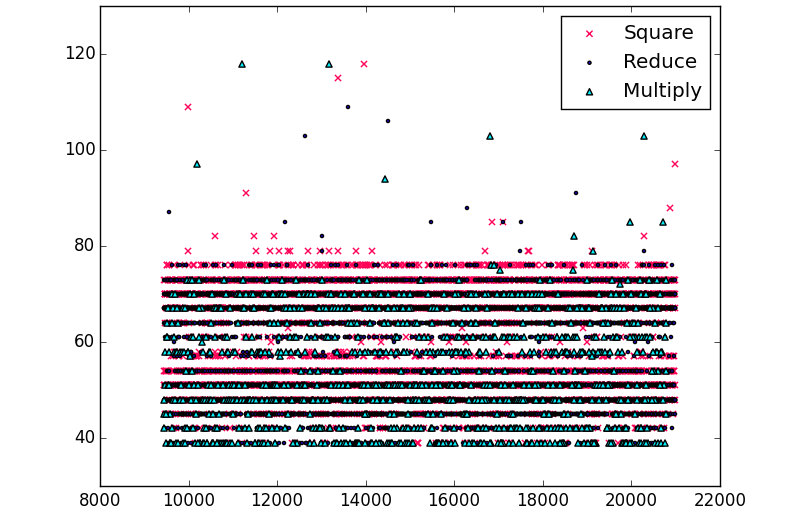
\includegraphics[width=\linewidth]{img/data/ec2}
  \caption{Overall timing graph from the EC2 instance}
  \label{fig:data-ec2}
\end{figure}

Results of a GPG signing session on a c3.large instance on Amazon EC2 seemed to
be the best (Figure~\ref{fig:data-ec2}). Looking at a small portion of the
chart, the sequence of squares, multiplications, and reductions becomes very
clear, as shown in Figure~\ref{fig:data-ec2-zoomed}.

\begin{figure}[h]
  \centering
    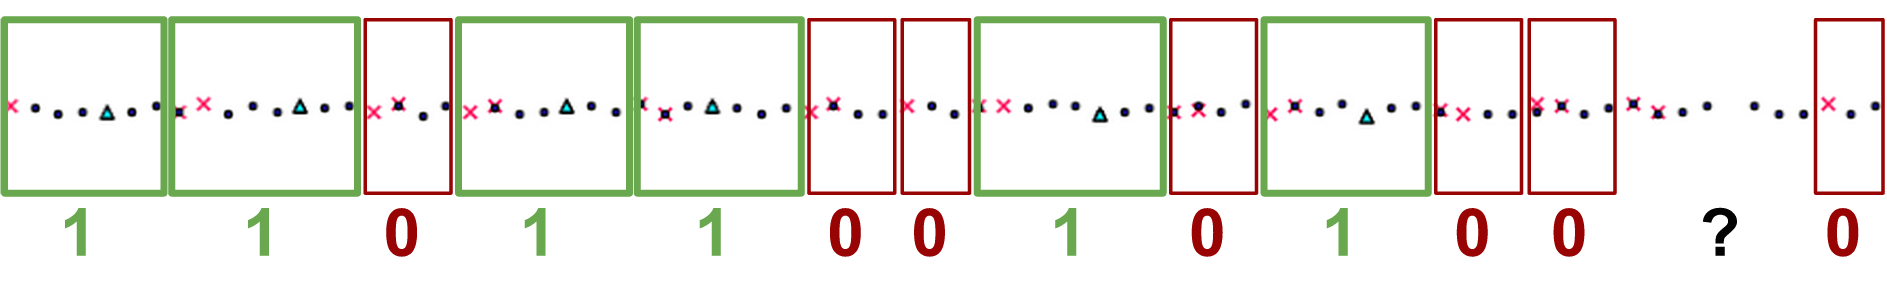
\includegraphics[width=\linewidth]{img/data/ec2-zoomed}
  \caption{Overall timing graph from the EC2 instance. This
  sequence of 0s and 1s is part of a larger 26-bit sequence that we were able to
  interpret and find in the 1023-bit $d_p$.}
  \label{fig:data-ec2-zoomed}
\end{figure}

Figure~\ref{fig:data-ec2-zoomed} shows that we can occasionally miss timings
when the OS schedules other processes in a time slot. Sometimes, this will make
that section of timings ambiguous; in this case, we could have either two
successive 0s or a single 1. The only way to resolve this ambiguity is capture
another GPG signing/decryption session with the same key and compare the
results.

\subsection{Other Platforms}

\subsubsection{OS X}

We were unable to extract any binary strings from the OS X results. However,
the output timing data looked promising and leads us to believe that OS X does
implement page deduplication. On many runs the
proportions of square, reduce, and multiplies were correct. A random assortment
of bits in the modulus combined with the access patterns of the algorithm should
produce a particular ratio, roughly $4:2:1$ reduces to squares to multiplies,
which we did observe. Furthermore, by tweaking the probe placement and
timing, the number of accesses observed per slot was between 1 and 2 on average,
which is close to the ideal of exactly one access per slot. Lastly, the banding
by cache level was very evident, similar to the EC2 results above. There was
little ambiguity about which probes resulted in cache hits and which did not.

As of writing, we did not examine the assembly of the GnuPG binary on OS X for
optimal probe placement; rather, we used the method of setting breakpoints in GDB by line
number and observing the addresses on which they were set. It is possible that
switching methods would produce better results.

\subsubsection{Arch Linux}

Arch Linux provided the poorest results by far. No meaningful data were
discernible under any configuration because there was too much timing noise
during the spying, which, in the case of the Figure~\ref{fig:data-arch}, occurred roughly
between timeslots 7000 and 18000 on the x-axis. Given that there were no
significant differences between this and the configuration running on OS X, we
were unsure why this kept occurring. The most obvious
difference between the two systems is that GnuPG on Arch Linux was compiled
under GCC 4.9.2 instead of GCC 4.2, as it was on OS X; however, it was not clear how
this would change the output so drastically, or if it did at all. Our two
hypotheses for this behaviour were that Arch Linux
was being run as a guest OS on a Windows 8.1 host, and that it was being run on
a Haswell-series Intel i7, which could have affected GCC's compilation of GnuPG
because this CPU series
did not exist at the publication time of the original paper.  However, both of
these hypotheses were disproven by testing on a second machine running Arch
Linux as a host OS on an older Intel Celeron CPU, in which the attack produced
the same noisy results.

\begin{figure}[h]
  \centering
    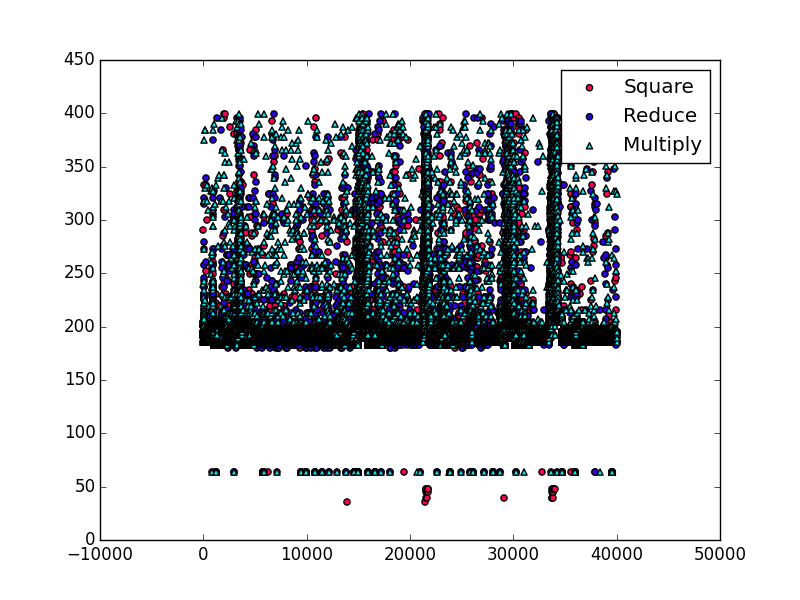
\includegraphics[width=\linewidth]{img/data/arch-graph-1}
  \caption{Overall timing graph from the Arch Linux setup.}
  \label{fig:data-arch}
\end{figure}

\subsection{Analysis}

Our results were quite sensitive to probe placement. The ideal probing addresses
are the ones that are always executed when the targeted operations
(\texttt{mpih\_sqr\_n\_basecase}, \texttt{mpihelp\_divrem}, and
\texttt{mpihelp\_mul\_karatsuba\_case}) are executed. Finding these addresses,
however, was not as straightforward as we thought it would be.

Since GPG is built with \texttt{-O2} optimzations, the assembly output does not
map one-to-one with the lines of source code; optimizations tend to do a
considerable amount of assembly ``jumbling'' (duplication, rearrangement, and
inlining of code). As a result, we found that setting probes to within
frequently accessed addresses, such as within loop bodies as suggested by Yarom
and Falkner\cite{YF13}, did not work as well as we expected.

Many of our preliminary results were plagued by a lot of noise, much of which
resulted from speculative execution. To reduce the effects of this, we attempted
to probe the very close to the ends of the respective functions. We found that
simply setting breakpoints to the relevant lines in GDB would not yield good
addresses to probe. Even setting a breakpoint to the last line of the function
in the source would not return an address of an instruction close to the return.
To find the best addresses, we disassembled the GPG binary using
\texttt{objdump} and located addresses near each function's \texttt{retq}
instruction.

\begin{lstlisting}[language={[x86masm]Assembler},
    caption={A probe at \texttt{0x08ed90} near the end of
    \texttt{mpihelp\_divrem}, the modulus function, on EC2 hardware.},float=*]
48ed90: add 0x78, %rsp	; probe set here
48ed94: pop %rbx
48ed95: pop %rbp
48ed96: pop %r12
48ed98: pop %r13
48ed9a: pop %r14
48ed9c: pop %r15
48ed9e: retq	; end of function, almost always executed
\end{lstlisting}

We developed a Python script to analyze the timing data. While the script was
able to recover many of the bits in $d_p$ and $d_q$, there were too many errors
in recovery preventing us from reliably reconstructing the private RSA exponent.
Further work will be needed to improve the robustness of the script.

\section{Conclusions}

We successfully reproduced parts of the \flushreload{} attack. While results
were mixed on various platforms, we found moderate success on EC2, which, in
particular, is an interesting environment vulnerable to this type of attack;
it shares hardware access with other guest VMs on the same host, opening the
possibility of a cross-VM attack. Although this vulnerability was fixed in GnuPG
version 1.4.14, this shows that other programs running on EC2 may be susceptible
to this technique.

We have endeavored to provide more details on some parts of the implementation
of this attack to reduce the barrier to future reproductions and
extensions of these results. Additionally, full source code is available upon
request.

\section{Future Work}

A possible future application of the \flushreload{} technique would be to
perform this attack across virtual machines. That is, using the attack to steal
data from one virtual machine whilst running the attack on another. Cross-VM
attacks are described in further detail by Apecechea et al.
\cite{cryptoeprint:2014:248}; the basic principle behind the attack would be to
detect and spy upon a victim, i.e. a user on another VM, running GnuPG (or some
equivalent cryptographic process) and steal the keys used in the process. Such
an attack clearly has its appeal: it would expose a major vulnerability in
virtual machines, which are used in countless modern software applications.

Alternatively, \flushreload{} could be used generally to spy on arbitrary
binaries, e.g.\ commonly-used binaries such as \texttt{ls}, \texttt{cd}, or
\texttt{cat}. By using \flushreload{} to probe the main functions of these
binaries, it is theoretically possible to determine the commands a user is
typing into their shell based on the timing of access to the instructions in the
binary. One could also put probes into the binary of a text editor such as
\texttt{vim} or \texttt{emacs}, and spy on the text a user is typing into said
editor. While no attack such as this currently exists, we could posit the
formulation of one like so: use \texttt{mmap} to map a given binary, and place
probes into the binary at particular locations. Probe locations can be chosen
simply by observing conditions upon which branches are taken and placing a probe
in each of the relevant branch targets, similar to how the attack on GnuPG
works.

\lobsectionbreak

\bibliographystyle{plain}
\bibliography{sources}

\hspace*{7cm} 
\lob[lobblue, scale=1.5]{83} \hfill

\end{document}
